% Poster version of DFT causal diagram — citation labels removed for readability at A0.
% Original (with citations): S2S_Thesis/figures/dft_causal_diagram.tex
% Compile with: pdflatex dft_causal_diagram_poster.tex

\documentclass[tikz,border=8pt]{standalone}
\usepackage[T1]{fontenc}
\usetikzlibrary{arrows.meta, positioning, calc, decorations.pathmorphing, backgrounds, fit}

% Bevacqua colour palette
\definecolor{modcol}{HTML}{F5C242}
\definecolor{drivcol}{HTML}{7AB648}
\definecolor{hazcol}{HTML}{4A90D9}
\definecolor{preccol}{HTML}{E8943A}
\definecolor{impcol}{HTML}{D94F4F}
\definecolor{phasebg}{HTML}{F7F7F7}

\begin{document}
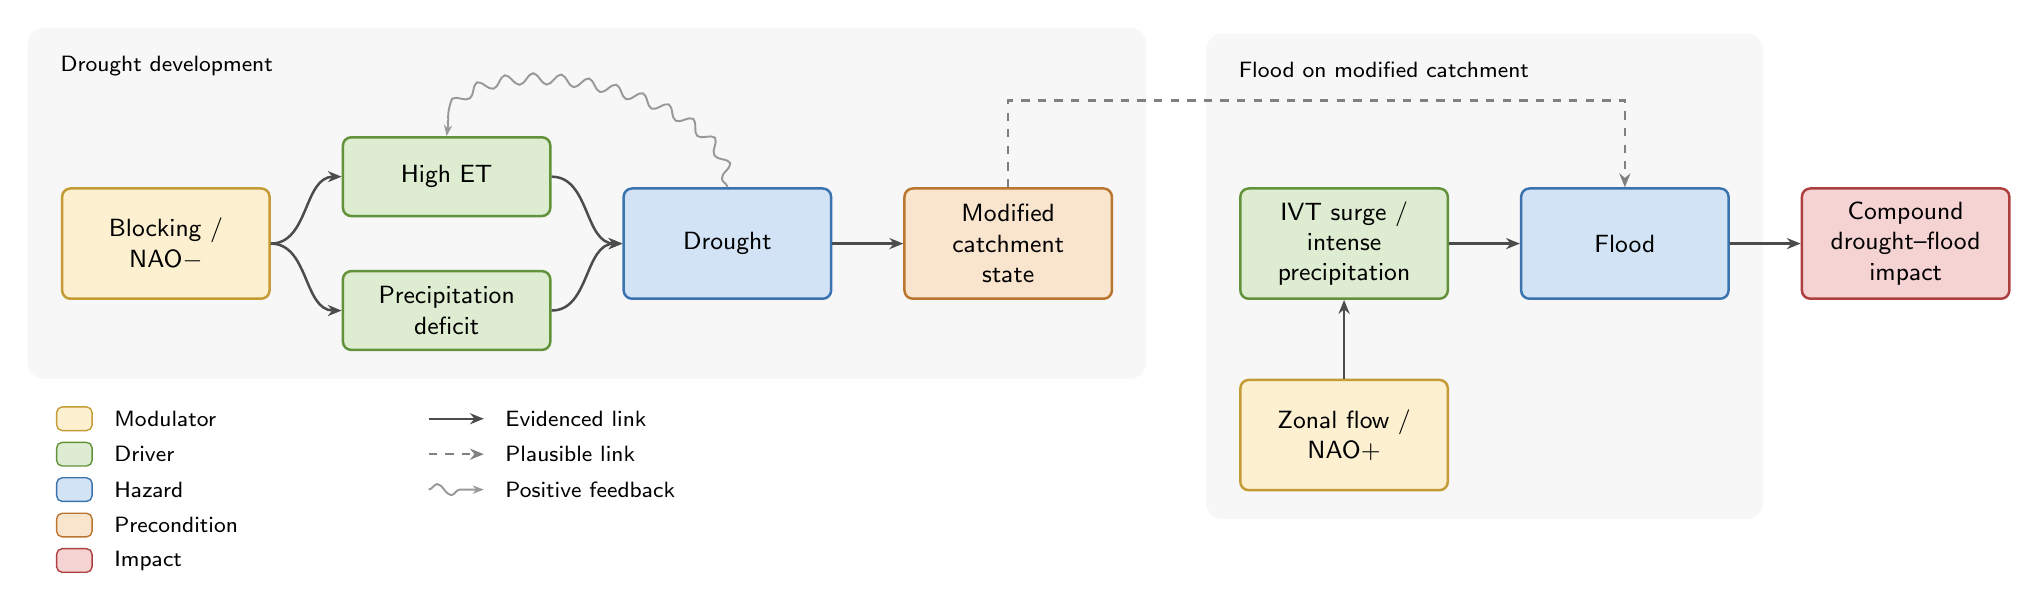
\begin{tikzpicture}[
    modbox/.style={
        rectangle, rounded corners=3pt, draw=modcol!80!black, line width=0.9pt,
        fill=modcol!25, minimum width=2.6cm, minimum height=1.4cm,
        text width=2.4cm, align=center, font=\small\sffamily
    },
    drivbox/.style={
        rectangle, rounded corners=3pt, draw=drivcol!80!black, line width=0.9pt,
        fill=drivcol!25, minimum width=2.6cm, minimum height=1.4cm,
        text width=2.4cm, align=center, font=\small\sffamily
    },
    hazbox/.style={
        rectangle, rounded corners=3pt, draw=hazcol!80!black, line width=0.9pt,
        fill=hazcol!25, minimum width=2.6cm, minimum height=1.4cm,
        text width=2.4cm, align=center, font=\small\sffamily
    },
    precbox/.style={
        rectangle, rounded corners=3pt, draw=preccol!80!black, line width=0.9pt,
        fill=preccol!25, minimum width=2.6cm, minimum height=1.4cm,
        text width=2.4cm, align=center, font=\small\sffamily
    },
    impbox/.style={
        rectangle, rounded corners=3pt, draw=impcol!80!black, line width=0.9pt,
        fill=impcol!25, minimum width=2.6cm, minimum height=1.4cm,
        text width=2.4cm, align=center, font=\small\sffamily
    },
    solid arrow/.style={
        -{Stealth[length=5pt, width=4pt]}, line width=0.9pt, color=black!70
    },
    dashed arrow/.style={
        -{Stealth[length=5pt, width=4pt]}, line width=0.9pt, color=black!50, dashed
    },
    feedback arrow/.style={
        -{Stealth[length=4pt, width=3pt]}, line width=0.7pt, color=black!40,
        decorate, decoration={snake, amplitude=0.7mm, segment length=3.5mm, post length=1.5mm}
    },
]

% ============================================================
% MAIN CHAIN
% ============================================================

% Drought development nodes
\node[modbox] (mod1) at (0, 0) {Blocking /\\NAO$-$};
\node[drivbox, right=0.9cm of mod1, yshift=0.85cm, minimum height=1.0cm] (driv1a) {High ET};
\node[drivbox, right=0.9cm of mod1, yshift=-0.85cm, minimum height=1.0cm] (driv1b) {Precipitation\\deficit};
\node[hazbox, right=0.9cm of driv1a, yshift=-0.85cm] (haz1) {Drought};
\node[precbox, right=0.9cm of haz1] (prec) {Modified\\catchment\\state};

% Flood on modified catchment nodes
\node[drivbox, right=1.6cm of prec] (driv2) {IVT surge /\\intense\\precipitation};
\node[hazbox, right=0.9cm of driv2] (haz2) {Flood};
\node[impbox, right=0.9cm of haz2] (imp) {Compound\\drought--flood\\impact};

% Phase 2 modulator
\node[modbox, below=1.0cm of driv2] (mod2) {Zonal flow /\\NAO$+$};

% ============================================================
% ARROWS
% ============================================================

\draw[solid arrow] (mod1.east) to[out=0, in=180] (driv1a.west);
\draw[solid arrow] (mod1.east) to[out=0, in=180] (driv1b.west);
\draw[solid arrow] (driv1a.east) to[out=0, in=180] (haz1.west);
\draw[solid arrow] (driv1b.east) to[out=0, in=180] (haz1.west);
\draw[solid arrow] (haz1) -- (prec);

\draw[dashed arrow]
    (prec.north) -- ++(0, 1.1)
    -| (haz2.north);

\draw[solid arrow] (driv2) -- (haz2);
\draw[solid arrow] (haz2) -- (imp);
\draw[solid arrow] (mod2) -- (driv2);

\draw[feedback arrow]
    (haz1.north) .. controls +(0, 1.2) and +(0, 1.2) .. (driv1a.north);

% ============================================================
% GREY PHASE BOXES
% ============================================================

\coordinate (boxtop1) at ($(mod1.north)+(0, 1.6)$);
\coordinate (boxtop2) at ($(driv2.north)+(0, 1.6)$);
\coordinate (fbcite) at ($(driv1a.north)!0.5!(haz1.north)+(0, 1.35)$);

\begin{pgfonlayer}{background}
    \node[fill=phasebg, rounded corners=6pt, inner xsep=12pt, inner ysep=10pt,
          fit=(mod1)(driv1a)(driv1b)(haz1)(prec)(boxtop1)(fbcite)] (phase1bg) {};

    \node[fill=phasebg, rounded corners=6pt, inner xsep=12pt, inner ysep=10pt,
          fit=(driv2)(haz2)(mod2)(boxtop2)] (phase2bg) {};
\end{pgfonlayer}

\node[font=\footnotesize\sffamily, text=black, anchor=north west]
    at ($(phase1bg.north west)+(0.3, -0.25)$) {Drought development};
\node[font=\footnotesize\sffamily, text=black, anchor=north west]
    at ($(phase2bg.north west)+(0.3, -0.25)$) {Flood on modified catchment};

% ============================================================
% LEGEND
% ============================================================

\node[rectangle, rounded corners=2pt, fill=modcol!25, draw=modcol!80!black,
      minimum width=0.45cm, minimum height=0.3cm, line width=0.5pt]
      (lg1) at ($(phase1bg.south west)+(0.6, -0.5)$) {};
\node[font=\footnotesize\sffamily, anchor=west] at ($(lg1.east)+(0.15, 0)$) {Modulator};

\node[rectangle, rounded corners=2pt, fill=drivcol!25, draw=drivcol!80!black,
      minimum width=0.45cm, minimum height=0.3cm, line width=0.5pt]
      (lg2) at ($(lg1)+(0, -0.45)$) {};
\node[font=\footnotesize\sffamily, anchor=west] at ($(lg2.east)+(0.15, 0)$) {Driver};

\node[rectangle, rounded corners=2pt, fill=hazcol!25, draw=hazcol!80!black,
      minimum width=0.45cm, minimum height=0.3cm, line width=0.5pt]
      (lg3) at ($(lg2)+(0, -0.45)$) {};
\node[font=\footnotesize\sffamily, anchor=west] at ($(lg3.east)+(0.15, 0)$) {Hazard};

\node[rectangle, rounded corners=2pt, fill=preccol!25, draw=preccol!80!black,
      minimum width=0.45cm, minimum height=0.3cm, line width=0.5pt]
      (lg4) at ($(lg3)+(0, -0.45)$) {};
\node[font=\footnotesize\sffamily, anchor=west] at ($(lg4.east)+(0.15, 0)$) {Precondition};

\node[rectangle, rounded corners=2pt, fill=impcol!25, draw=impcol!80!black,
      minimum width=0.45cm, minimum height=0.3cm, line width=0.5pt]
      (lg5) at ($(lg4)+(0, -0.45)$) {};
\node[font=\footnotesize\sffamily, anchor=west] at ($(lg5.east)+(0.15, 0)$) {Impact};

\coordinate (arrcol) at ($(lg1)+(4.5, 0)$);

\draw[solid arrow] (arrcol) -- ++(0.7, 0);
\node[font=\footnotesize\sffamily, anchor=west] at ($(arrcol)+(0.85, 0)$) {Evidenced link};

\draw[dashed arrow] ($(arrcol)+(0, -0.45)$) -- ++(0.7, 0);
\node[font=\footnotesize\sffamily, anchor=west] at ($(arrcol)+(0.85, -0.45)$) {Plausible link};

\draw[feedback arrow] ($(arrcol)+(0, -0.9)$) -- ++(0.7, 0);
\node[font=\footnotesize\sffamily, anchor=west] at ($(arrcol)+(0.85, -0.9)$) {Positive feedback};

\end{tikzpicture}
\end{document}
